\documentclass[12pt, letterpaper]{article}
\usepackage{graphicx} % Required for inserting images
\usepackage{amsmath}
\usepackage{mdframed}

\title{telegraph equations solved with MFEM library using MFEM}
\author{Denis Lachapelle}
\date{May 2025}

\setlength{\parindent}{0pt}

\begin{document}

\maketitle

\section{Introduction}
This document explains the telegraph equations simulation using finite difference method based on MFEM library.

\section{Theory}

\subsection{From Telegrah PDE to Matrix form}

The telegraph equations are:

  \begin{equation}\frac{\partial{V}}{\partial{x}} + L \frac{\partial{I}}{\partial{t}} + R I = 0\end{equation}


\begin{equation}\frac{\partial{I}}{\partial{x}} + C \frac{\partial{V}}{\partial{t}} + G V = 0\end{equation}

For now assumes a single line from points a to b.\\

Going to weak form using different space for V and I, $\phi$ for V and $\psi$ for I. Note the test functions span the entire domain and is zero on the border and the equations below have to be true for all test functions. Look at "element\_finis.pdf" p. 42.

\begin{equation}\int_\Omega(\frac{\partial{V}}{\partial{x}} + L \frac{\partial{I}}{\partial{t}} + R I) \phi = 0\end{equation}

\begin{equation}\int_\Omega(\frac{\partial{I}}{\partial{x}} + C \frac{\partial{V}}{\partial{t}} + G V) \psi = 0\end{equation}

and then


\begin{equation}
\int_\Omega\frac{\partial{V}}{\partial{x}} \phi
+ \int_\Omega(L \frac{\partial{I}}{\partial{t}} +  R I) \phi
= 0
\end{equation}



\begin{equation}
\int_\Omega\frac{\partial{I}}{\partial{x}} \psi
+ \int_\Omega(C \frac{\partial{V}}{\partial{t}} +  G V) \psi
= 0
\end{equation}

Using integration by part on the first term...

\begin{equation}\int_a^b u(x) v'(x) \, dx = \Big[u(x) v(x)\Big]_a^b - \int_a^b u'(x) v(x) \, dx\end{equation}

Each equations becomes ...

\begin{equation}
\Big[\phi V \Big]_a^b
-\int_\Omega(V \frac{\partial{\phi}}{\partial{x}})
+ \int_\Omega(L \frac{\partial{I}}{\partial{t}} +  R I) \phi
= 0
\end{equation}

\begin{equation}\Big[\psi I \Big]_a^b
-\int_\Omega(I \frac{\partial{\psi}}{\partial{x}})
+ \int_\Omega(C \frac{\partial{V}}{\partial{t}} +  G V) \psi
= 0
\end{equation}

Then we approximate by different basis function for V and I, V(x) by

\begin{equation}V(x) = \sum_j V_j \phi(x) \end{equation}

and I(x) by 

\begin{equation}I(x) = \sum_j I_j \psi(x) \end{equation}

Where $I_j$ and $V_j$ are constants and notice that $\Big[\phi V \Big]_a^b$ and $\Big[\psi I \Big]_a^b$ are zero since $\phi$ and $\psi$ are zero on the border.\\

Equations (8) becomes ...

\begin{equation}
	\int_{\Omega_i} \sum_j V_j \phi_j \frac{\partial{\phi_i}}{\partial{x}} 
	- L \int_{\Omega_i} \frac{\partial{}}{\partial t} \Big[ \sum{I_j} \psi_j \Big] \phi_i
	-  R \int_{\Omega_i} \sum_j I_j \psi_j \phi_i
	= 0
\end{equation}

Assume $\frac{\partial{I}}{\partial{t}}$ is constant on each element so we can exclude $\frac{\partial{I}}{\partial{t}}$ from inside the integral and interchange the integral and summation.

\begin{equation}
	\sum_j V_j \int_{\Omega_i}\phi_j \frac{\partial{\phi_i}}{\partial{x}} 
	- L \sum_j \frac{\partial{I_j}}{\partial t} \int_{\Omega_i} \psi_j \phi_i
	-  R \sum_j I_j \int_{\Omega_i} \psi_j \phi_i
	= 0
\end{equation}

and equation 9 becomes ...

\begin{equation}
	\sum_j I_j  \int_\Omega \psi_j \frac{\partial{\psi_i}}{\partial{x}}
	- C \sum_j \frac{\partial{V_j}}{\partial{t}} \int_\Omega \phi_j \psi_i
	- G \sum_j V_j \int_\Omega \phi_j \psi_i
	= 0
\end{equation}

So now we have two equations (13) and (14) with unknown $V_j$ and $I_j$.\\

The j span the trial functions (Approximating Functions) and the i span the elements. The equations can be converted in matrix form...

\begin{equation}
	S_V V - L M_V \frac{\partial I}{\partial t} - R M_V I = 
	= 0
\end{equation}

\begin{equation}
	S_I I - C M_I \frac{\partial V}{\partial t} - G M_I V = 
	= 0
\end{equation}

Where ...

\[S_V = \int_\Omega \phi_j \frac{\partial \phi_i}{\partial x}\]
dimensions VDOFxVDOF

\[M_V = \int_\Omega \psi_j \phi_i\]
dimension VDOFxIDOF

\[S_I = \int_\Omega \psi_j \frac{\partial \psi_i}{\partial x}\]
dimension IDOFxIDOF

\[M_I = \int_\Omega \phi_j \psi_i\]
dimension IDOFxVDOF\\

Note that $S_V = S_I^T$.\\

In equations 13 and 14 we have $\frac{\partial V}{\partial t}$ and $\frac{\partial I}{\partial t}$ that can each be approximated by $\frac{I_{n+1}-I_n}{\Delta t}$. This is the forward Euler method (explicit Euler method).

\begin{equation}
	S_V V_n - L M_V (\frac{I_{n+1}-I_n}{\Delta t}) - R M_V I_n
	= 0
\end{equation}

\begin{equation}
	S_I I_n - C M_I (\frac{V_{n+1}-V_n}{\Delta t}) - G M_I V_n = 
	= 0
\end{equation}


Now with $V_{n+1}$ and $I_{n+1}$ on the left side.

\begin{equation}
	V_{n+1} = V_n + \frac{1}{C} M_I^{-1} S_I I_n \Delta t - \frac{G}{C} V_n \Delta t
\end{equation}

\begin{equation}
	I_{n+1} =  I_n + \frac{1}{L} M_V^{-1} S_V V_n \Delta t - \frac{R}{L} I_n \Delta t
\end{equation}

The above solution is not appropriated since $M_V$ and $M_I$ are not square and thus cannot be inverted.
\\
\\
Note they are not square because the trial and test functions are not the same (not so sure here).


\subsection{another way without matrix inversion}
Starting from equation 17 and 18.

\begin{equation}
	S_V V_n - \frac{L M_V}{\Delta t} I_{n+1} + \frac{L M_V}{\Delta t} I_n - R M_V I_n
	= 0
\end{equation}

\begin{equation}
	S_I I_n - \frac{C M_I}{\Delta t} V_{n+1} + \frac{C M_I}{\Delta t} V_n - G M_I V_n = 
	= 0
\end{equation}

\begin{equation}
	\frac{L M_V}{\Delta t} I_{n+1} = \frac{L M_V}{\Delta t} I_n - R M_V I_n + S_V V_n
\end{equation}

\begin{equation}
	\frac{C M_I}{\Delta t} V_{n+1}
	= \frac{C M_I}{\Delta t} V_n - G M_I V_n + S_I I_n 
\end{equation}

\begin{equation}
	M_V I_{n+1} = M_V I_n - \frac{R \Delta t}{L} M_V I_n + \frac{\Delta t}{L} S_V V_n
\end{equation}

\begin{equation}
	M_I V_{n+1}
	= M_I V_n - \frac{G \Delta t}{C} M_I V_n + \frac{\Delta t}{C} S_I I_n 
\end{equation}


\begin{equation}
	M_V I_{n+1} = (1 - \frac{R \Delta t}{L}) M_V I_n + \frac{\Delta t}{L} S_V V_n
\end{equation}

\begin{equation}
	M_I V_{n+1}
	= (1 - \frac{G \Delta t}{C}) M_I V_n + \frac{\Delta t}{C} S_I I_n 
\end{equation}


\subsection{Boundary}
Now we have a voltage source $V_S$ driving transmission line point a through a resistor of $R_S$ ohm.

\begin{equation}
R_S I_a + V_a = V_S
\end{equation}

The transmission line point b is loaded with a resistor $R_L$.

\begin{equation}
V_b - R_L I_b = 0
\end{equation}


\subsection{The complete Matrix System}


\begin{equation}
	V_{a,n+1} = V_S - R_S I_{a,n}
\end{equation}

\begin{equation}
	V_{b,n+1} = R_L I_{b,n}
\end{equation}


The system is a block matrix 

\begin{equation}
	\begin{bmatrix}
		M_I & 0 \\
		0   & M_V
	\end{bmatrix}
	\begin{bmatrix}
		V_{n+1} \\
		I_{n+1} \\
	\end{bmatrix}
	=
	\begin{bmatrix}
	K3 M_I & K4 S_I\\
	K1 S_V & K2 M_V
		
	\end{bmatrix}
	\begin{bmatrix}
		V_{n} \\
		I_{n} \\
	\end{bmatrix}
\end{equation}

Where ...

\[K1 = \frac{\Delta t}{L}\]
\[K2 = 1 - \frac{R \Delta t}{L}\]
\[K3 = 1 - \frac{G \Delta t}{C}\]
\[K4 = \frac{\Delta t}{C}\]


Here we still have to include the Vs and load.\\

To include $V_S$ and $R_S$ we should add a column $\begin{Bmatrix} 1 & 0 $ 0 $ 0 $ ... $ 0\end{Bmatrix}^T$ on the rhs matrix and $V_S$ to the rhs column vector and replace the first row of $K4 S_I$ by $\begin{Bmatrix} -R_S & 0 $ 0 $ 0 $ ... $ 0\end{Bmatrix}$ and zeroed the first row of $K3 M_I$ to match equation 31.

\begin{equation}
	\begin{bmatrix}
		M_I & 0\\
		0 & M_V 
	\end{bmatrix}
	\begin{bmatrix}
		V_{n+1} \\
		I_{n+1} \\
	\end{bmatrix}
	=
	\begin{bmatrix}
		1 & K3 M_I & K4 S_I \\
		0 & K1 S_V & K2 M_V
	\end{bmatrix}
	\begin{bmatrix}
		V_S \\
		V_{n} \\
		I_{n} \\
	\end{bmatrix}
\end{equation}

Now to include the load $R_L$ zeroed the last row of $K3 M_I$ and replaced the last row of $K4 S_I$ by $\begin{Bmatrix} 0 & 0 $ 0 $ 0 $ ... $ R_L\end{Bmatrix}$.\\

Now check if the size of each matrix make sense.

\begin{equation}
	\begin{bmatrix}
		IxV & 0 \\
		0 & VxI
	\end{bmatrix}
	\begin{bmatrix}
		Vx1 \\
		Ix1 
	\end{bmatrix}
	=
	\begin{bmatrix}
		1 & IxV & IxI \\
		0 & VxV & VxI
	\end{bmatrix}
	\begin{bmatrix}
		1x1 \\
		Vx1 \\
		Ix1 \\
	\end{bmatrix}
\end{equation}

Once the matrix multiplication done

\begin{equation}
	\begin{bmatrix}
		Ix1 \\
		Vx1 
	\end{bmatrix}
	=
	\begin{bmatrix}
		Ix1 \\
		Vx1
	\end{bmatrix}
\end{equation}

So it look fine since the dimensions match.

\section{MFEM Implementation}

With the theory developed above we can start implementing the program using MFEM\footnote{https://mfem.org/} library.

The program is named stlt.cpp for single transmission line transient.

The program will run this way:


\begin{enumerate}
	\item Compute the two block matrix, the lhs and the rhs.
	
	\begin{enumerate}
		\item matrice $M_V$, $M_I$, $S_V$ and $S_I$ computed.
		\item rhs and lhs matrices assembled as block operator.
		\item RS and RL included in the system.
		\item VS ???
		\end{enumerate}	
	\item compute $V_S$ at the time $n \Delta t$
	\item compute the rhs by matrix multiplication.
	\item solve the system of equations
\end{enumerate}

 \begin{equation}
 	\begin{bmatrix}
 		lhsOp
 	\end{bmatrix}
 	\begin{bmatrix}
 		xL
 	\end{bmatrix}
 	=
 	\begin{bmatrix}
 		rhsOp
 	\end{bmatrix}
 	\begin{bmatrix}
 		xR
 	\end{bmatrix}
 \end{equation}

 \begin{equation}
	\begin{bmatrix}
		lhsOp
	\end{bmatrix}
	\begin{bmatrix}
		xL
	\end{bmatrix}
	=
	\begin{bmatrix}
		y
	\end{bmatrix}
\end{equation}




\begin{mdframed}
The system is unstable... try with deltaT = 0.01e-9 instead of 0.1 e-9.\\
Change L, C, R and G for RG-58.\\
// Constants for the telegrapher’s equation for RG-58, 50 ohm.\\
double L = 250e-9;  // Inductance per unit length\\
double C = 100.0e-12; // Capacitance per unit length\\
double R = 10e-3;  // Resistance per unit length\\
double G = 1.0e-9;  // Conductance per unit length.\\
\\
I find some problem in the matrix system theory, so I change the stucture.\\
So i need to adjust the software.\\

The determinant of the $\begin{bmatrix} lhsOp \end{bmatrix}$ is zero and the condition number is very high, so it wont converge.
  \end{mdframed}
  
  
  \section{Theory, a second trial}
  Assuming both V and I in H1 space, this will make $M_I$ and $M_V$ square, it will then be possible to invert them.
  
  \subsection{From Telegrah PDE to Matrix form}
  
  The telegraph equations are:
  
  \begin{equation}\frac{\partial{V}}{\partial{x}} + L \frac{\partial{I}}{\partial{t}} + R I = 0\end{equation}
  
  
  \begin{equation}\frac{\partial{I}}{\partial{x}} + C \frac{\partial{V}}{\partial{t}} + G V = 0\end{equation}
  
  For now assumes a single line from points a to b.\\
  
Going to weak form using same space for V and I. Note the test functions span the entire domain and is zero on the border and the equations below have to be true for all test functions. Look at "element\_finis.pdf" p. 42.

\begin{equation}\int_\Omega(\frac{\partial{V}}{\partial{x}} + L \frac{\partial{I}}{\partial{t}} + R I) \phi = 0\end{equation}

\begin{equation}\int_\Omega(\frac{\partial{I}}{\partial{x}} + C \frac{\partial{V}}{\partial{t}} + G V) \phi = 0\end{equation}

and then


\begin{equation}
	\int_\Omega\frac{\partial{V}}{\partial{x}} \phi
	+ \int_\Omega(L \frac{\partial{I}}{\partial{t}} +  R I) \phi
	= 0
\end{equation}



\begin{equation}
	\int_\Omega\frac{\partial{I}}{\partial{x}} \phi
	+ \int_\Omega(C \frac{\partial{V}}{\partial{t}} +  G V) \phi
	= 0
\end{equation}

Using integration by part on the first term...

\begin{equation}\int_a^b u(x) v'(x) \, dx = \Big[u(x) v(x)\Big]_a^b - \int_a^b u'(x) v(x) \, dx\end{equation}

Each equations becomes ...

\begin{equation}
	\Big[\phi V \Big]_a^b
	-\int_\Omega(V \frac{\partial{\phi}}{\partial{x}})
	+ \int_\Omega(L \frac{\partial{I}}{\partial{t}} +  R I) \phi
	= 0
\end{equation}

\begin{equation}\Big[\phi I \Big]_a^b
	-\int_\Omega(I \frac{\partial{\phi}}{\partial{x}})
	+ \int_\Omega(C \frac{\partial{V}}{\partial{t}} +  G V) \phi
	= 0
\end{equation}

Then we approximate V and I, V(x) by

\begin{equation}V(x, t) = \sum_j V_j(t) \phi(x) \end{equation}

and I(x) by 

\begin{equation}I(x, t) = \sum_j I_j(t) \phi(x) \end{equation}

Notice that $\Big[\phi V \Big]_a^b$ and $\Big[\phi I \Big]_a^b$ are zero since $\phi$ is zero on the border.\\

Equations (46) becomes ...

\begin{equation}
	\int_{\Omega_i} \sum_j V_j \phi_j \frac{\partial{\phi_i}}{\partial{x}} 
	- L \int_{\Omega_i} \frac{\partial{}}{\partial t} \Big[ \sum{I_j} \phi_j \Big] \phi_i
	-  R \int_{\Omega_i} \sum_j I_j \phi_j \phi_i
	= 0
\end{equation}

Assume $\frac{\partial{I}}{\partial{t}}$ is constant on each element so we can exclude $\frac{\partial{I}}{\partial{t}}$ from inside the integral and interchange the integral and summation.

\begin{equation}
	\sum_j V_j \int_{\Omega_i}\phi_j \frac{\partial{\phi_i}}{\partial{x}} 
	- L \sum_j \frac{\partial{I_j}}{\partial t} \int_{\Omega_i} \phi_j \phi_i
	-  R \sum_j I_j \int_{\Omega_i} \phi_j \phi_i
	= 0
\end{equation}

and equation 9 becomes ...

\begin{equation}
	\sum_j I_j  \int_\Omega \phi_j \frac{\partial{\phi_i}}{\partial{x}}
	- C \sum_j \frac{\partial{V_j}}{\partial{t}} \int_\Omega \phi_j \phi_i
	- G \sum_j V_j \int_\Omega \phi_j \phi_i
	= 0
\end{equation}

So now we have two equations (51) and (52) with unknown $V_j(t)$ and $I_j(t)$.\\

The j span the trial functions (Approximating Functions) and the i span the elements. The equations can be converted in matrix form...

\begin{equation}
	S_V V - L M_V \frac{\partial I}{\partial t} - R M_V I = 
	= 0
\end{equation}

\begin{equation}
	S_I I - C M_I \frac{\partial V}{\partial t} - G M_I V = 
	= 0
\end{equation}

Where ...

\[S_V = \int_\Omega \phi_j \frac{\partial \phi_i}{\partial x}\]
dimensions VDOFxVDOF

\[M_V = \int_\Omega \phi_j \phi_i\]
dimension VDOFxIDOF

\[S_I = \int_\Omega \phi_j \frac{\partial \phi_i}{\partial x}\]
dimension IDOFxIDOF

\[M_I = \int_\Omega \phi_j \phi_i\]
dimension IDOFxVDOF\\


In equations 53 and 54 we have $\frac{\partial V}{\partial t}$ and $\frac{\partial I}{\partial t}$ that can each be approximated by $\frac{I_{n+1}-I_n}{\Delta t}$. This is the forward Euler method (explicit Euler method).

\begin{equation}
	S_V V_n - L M_V (\frac{I_{n+1}-I_n}{\Delta t}) - R M_V I_n
	= 0
\end{equation}

\begin{equation}
	S_I I_n - C M_I (\frac{V_{n+1}-V_n}{\Delta t}) - G M_I V_n = 
	= 0
\end{equation}


Now with $V_{n+1}$ and $I_{n+1}$ on the left side.

\begin{equation}
	V_{n+1} = V_n + \frac{1}{C} M_I^{-1} S_I I_n \Delta t - \frac{G}{C} V_n \Delta t
\end{equation}

\begin{equation}
	I_{n+1} =  I_n + \frac{1}{L} M_V^{-1} S_V V_n \Delta t - \frac{R}{L} I_n \Delta t
\end{equation}

\subsection{another way without matrix inversion}
Starting from equation 17 and 18.

\begin{equation}
	S_V V_n - \frac{L M_V}{\Delta t} I_{n+1} + \frac{L M_V}{\Delta t} I_n - R M_V I_n
	= 0
\end{equation}

\begin{equation}
	S_I I_n - \frac{C M_I}{\Delta t} V_{n+1} + \frac{C M_I}{\Delta t} V_n - G M_I V_n = 
	= 0
\end{equation}

\begin{equation}
	\frac{L M_V}{\Delta t} I_{n+1} = \frac{L M_V}{\Delta t} I_n - R M_V I_n + S_V V_n
\end{equation}

\begin{equation}
	\frac{C M_I}{\Delta t} V_{n+1}
	= \frac{C M_I}{\Delta t} V_n - G M_I V_n + S_I I_n 
\end{equation}

\begin{equation}
	M_V I_{n+1} = M_V I_n - \frac{R \Delta t}{L} M_V I_n + \frac{\Delta t}{L} S_V V_n
\end{equation}

\begin{equation}
	M_I V_{n+1}
	= M_I V_n - \frac{G \Delta t}{C} M_I V_n + \frac{\Delta t}{C} S_I I_n 
\end{equation}


\begin{equation}
	M_V I_{n+1} = (1 - \frac{R \Delta t}{L}) M_V I_n + \frac{\Delta t}{L} S_V V_n
\end{equation}

\begin{equation}
	M_I V_{n+1}
	= (1 - \frac{G \Delta t}{C}) M_I V_n + \frac{\Delta t}{C} S_I I_n 
\end{equation}

These two equations are more appropriated since we will use a solver.

\subsection{Boundary}
Now we have a voltage source $V_S$ driving transmission line point a through a resistor of $R_S$ ohm.

\begin{equation}
	R_S I_a + V_a = V_S
\end{equation}

The transmission line point b is loaded with a resistor $R_L$.

\begin{equation}
	V_b - R_L I_b = 0
\end{equation}


\subsection{The complete Matrix System}


\begin{equation}
	V_{a,n+1} = V_S - R_S I_{a,n}
\end{equation}

\begin{equation}
	V_{b,n+1} = R_L I_{b,n}
\end{equation}


The system is a block matrix 

\begin{equation}
	\begin{bmatrix}
		M_I & 0 \\
		0   & M_V
	\end{bmatrix}
	\begin{bmatrix}
		V_{n+1} \\
		I_{n+1} \\
	\end{bmatrix}
	=
	\begin{bmatrix}
		K3 M_I & K4 S_I\\
		K1 S_V & K2 M_V
		
	\end{bmatrix}
	\begin{bmatrix}
		V_{n} \\
		I_{n} \\
	\end{bmatrix}
\end{equation}

Where ...

\[K1 = \frac{\Delta t}{L}\]
\[K2 = 1 - \frac{R \Delta t}{L}\]
\[K3 = 1 - \frac{G \Delta t}{C}\]
\[K4 = \frac{\Delta t}{C}\]


Here we still have to include the Vs and load.\\

To include $V_S$ and $R_S$ we should add a column $\begin{Bmatrix} 1 & 0 $ 0 $ 0 $ ... $ 0\end{Bmatrix}^T$ on the rhs matrix and $V_S$ to the rhs column vector and replace the first row of $K4 S_I$ by $\begin{Bmatrix} -R_S & 0 $ 0 $ 0 $ ... $ 0\end{Bmatrix}$ and zeroed the first row of $K3 M_I$ to match equation 31.

\begin{equation}
	\begin{bmatrix}
		M_I & 0\\
		0 & M_V 
	\end{bmatrix}
	\begin{bmatrix}
		V_{n+1} \\
		I_{n+1} \\
	\end{bmatrix}
	=
	\begin{bmatrix}
		1 & K3 M_I & K4 S_I \\
		0 & K1 S_V & K2 M_V
	\end{bmatrix}
	\begin{bmatrix}
		V_S \\
		V_{n} \\
		I_{n} \\
	\end{bmatrix}
\end{equation}

Now to include the load $R_L$ zeroed the last row of $K3 M_I$ and replaced the last row of $K4 S_I$ by $\begin{Bmatrix} 0 & 0 $ 0 $ 0 $ ... $ R_L\end{Bmatrix}$.\\


\section{MFEM Implementation}

With the theory developed above we can start implementing the program using MFEM\footnote{https://mfem.org/} library.

The program is named stltfe.cpp for single transmission line transient forward euler.

The program will run this way:


\begin{enumerate}
	\item Compute the two block matrix, the lhs and the rhs.
	
	\begin{enumerate}
		\item matrice $M_V$, $M_I$, $S_V$ and $S_I$ computed.
		\item rhs and lhs matrices assembled as block operator.
		\item RS and RL included in the system.
		\item VS ???
	\end{enumerate}	
	\item compute $V_S$ at the time $n \Delta t$
	\item compute the rhs by matrix multiplication.
	\item solve the system of equations
\end{enumerate}

\begin{equation}
	\begin{bmatrix}
		lhsOp
	\end{bmatrix}
	\begin{bmatrix}
		xL
	\end{bmatrix}
	=
	\begin{bmatrix}
		rhsOp
	\end{bmatrix}
	\begin{bmatrix}
		xR
	\end{bmatrix}
\end{equation}

\begin{equation}
	\begin{bmatrix}
		lhsOp
	\end{bmatrix}
	\begin{bmatrix}
		xL
	\end{bmatrix}
	=
	\begin{bmatrix}
		b
	\end{bmatrix}
\end{equation}




\begin{mdframed}
	The system is unstable even if i remove the source and apply an initial condition of 1,
\end{mdframed}

\section{Theory, Finite Differences}

The telegraph equations are:

\begin{equation}\frac{\partial{V}}{\partial{x}} + L \frac{\partial{I}}{\partial{t}} + R I = 0\end{equation}


\begin{equation}\frac{\partial{I}}{\partial{x}} + C \frac{\partial{V}}{\partial{t}} + G V = 0\end{equation}


\begin{enumerate}
\item Assume the TL is divided in N segments with node 0 to N. There is N+1 nodes.
\item Assume the $\frac{\partial V(t, x)}{\partial x}$ and $\frac{\partial I(t, x)}{\partial x}$ are constant over each segment.
\end{enumerate}

So at a given time t we can express the $\frac{\partial V(t, x)}{\partial x}$ and $\frac{\partial I(t, x)}{\partial x}$ as difference  $\frac{V(t, n h) - V(t, (n-1) h)}{h}$ and  $\frac{I(t, n h) - I(t, (n-1) h)}{h}$.

We can write matrix equations....

\begin{equation}
\frac{\partial{I}}{\partial{t}} 
=
	\begin{bmatrix}
		Dv & Ri
	\end{bmatrix}
	\begin{bmatrix}
		V^k \\
		I^k \\
	\end{bmatrix}
\end{equation}

\begin{equation}
	\frac{\partial{V}}{\partial{t}} 
	=
	\begin{bmatrix}
		Gv & Di
	\end{bmatrix}
	\begin{bmatrix}
		V^k \\
		I^k \\
	\end{bmatrix}
\end{equation}

The two equations above can be written as a single matrix equation...

\begin{equation}
    \begin{bmatrix}
    	\frac{\partial{V}}{\partial{t}} \\
    	\frac{\partial{I}}{\partial{t}} 
    \end{bmatrix}	
	=
	\begin{bmatrix}
		Gv Di \\
		Dv Ri
	\end{bmatrix}
	\begin{bmatrix}
		V^k \\
		I^k \\
	\end{bmatrix}
\end{equation}


\begin{equation}
	\begin{bmatrix}
		V^{k+1} \\
		I^{k+1} \\
	\end{bmatrix}
	=
	\begin{bmatrix}
		V^k \\
		I^k \\
	\end{bmatrix}
	+
	\Delta t
\begin{bmatrix}
	\frac{\partial{V}}{\partial{t}} \\
	\frac{\partial{I}}{\partial{t}} 
\end{bmatrix}	
\end{equation}

\begin{equation}
	\begin{bmatrix}
		V^{k+1} \\
		I^{k+1} \\
	\end{bmatrix}
	=
	\begin{bmatrix}
		V^k \\
		I^k \\
	\end{bmatrix}
	+
	\Delta t
	\begin{bmatrix}
		Gv Di \\
		Dv Ri
	\end{bmatrix}
	\begin{bmatrix}
		V^k \\
		I^k \\
	\end{bmatrix}	
\end{equation}


Where Dv and Di are the same derivative matrix multiplied by different terms -1/L for Dv and -1/C for Di.

\begin{equation}
	\begin{bmatrix}
	   -1/h & 1/h & 0 & 0 & ... &0 &0 \\
	   0 &-1/h & 1/h& 0 &... &0 &0 \\
	   0& 0& -1/h &1/h &... &0 &0 \\
	   0& 0& 0& -1/h &1/h & ... &0 \\
	   0& 0& 0&... &0 &-1/h &1/h  \\
	   0& 0& 0&... &0 & -1/h &1/h  \\
	\end{bmatrix}
\end{equation}

Gv and Ri are identity matrix scale by either -G/C and -R/L.

For Dv the multiplier value will be $\frac{\Delta t}{L h}$ which is in our case 1e-12/(250e-9 1e-3) = 0.004

\subsection{MFEM Implementation}

The program is named stltfd.cpp for Single Transmission Line Transient Finite Difference.

No way to get the stable, signal do not make sense. Try with a step, impulse and a sine wave 1 Ghz.

\begin{figure}[h]
	\centering
	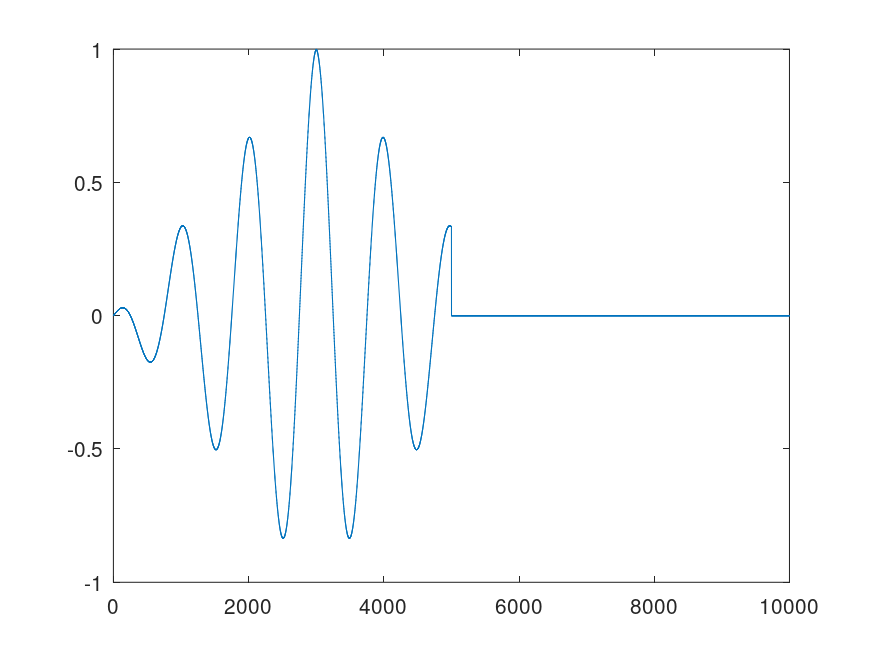
\includegraphics[width=0.8\textwidth]{testpulse_1.png} % Adjust width as needed
	\caption{Test pulse}
	\label{fig:example}
\end{figure}

I try with central difference and same problem.

I read that backward Euler and Crank-Nicolson are more stable.

Should I try with python? I have doubt about MFEM.

I made some test and the Dv and Di matrix within the block matrix works fine.

For Dv the multiplier value will be $\frac{\Delta t}{L h}$ which is in our case 1e-12/(250e-9 1e-3) = 0.004.

For Di the multiplier value will be $\frac{\Delta t}{C h}$ which is in our case 1e-12/(100e-12 1e-3) = 10.



\section{Another way, Finite Difference Discretization}

\subsection{Discretizing the first equation}

$V_i^n$ is meaning $V_{i h}^{n \Delta t}$

\begin{equation}
	\frac{V_{i+1}^n - V_i^n}{\Delta x} + L \frac{I_i^{n+1} - I_i^n}{\Delta t} + R I_i^n = 0
\end{equation}

Rearranged for \( I_i^{n+1} \):

\begin{equation}
	I_i^{n+1} = I_i^n - \frac{\Delta t}{L} \left( \frac{V_{i+1}^n - V_i^n}{\Delta x} + R I_i^n \right)
\end{equation}

\subsection{Discretizing the second equation}

\begin{equation}
	\frac{I_{i+1}^n - I_i^n}{\Delta x} + C \frac{V_i^{n+1} - V_i^n}{\Delta t} + G V_i^n = 0
\end{equation}

Rearranged for \( V_i^{n+1} \):

\begin{equation}
	V_i^{n+1} = V_i^n - \frac{\Delta t}{C} \left( \frac{I_{i+1}^n - I_i^n}{\Delta x} + G V_i^n \right)
\end{equation}

\section{Conclusion (for now: April 6, 2025)}
I never succeed in any way; I may be confused with the expected result or the stability. I start trying with finite method and then finite difference, none succeeded.\\

Given my many reading, the finite element method is one of the best with the finite volume method. I suspect the code I made for finite element method using MFEM is mostly right, but I do not provide valid initial and boundary conditions and my understanding of the output was not good.\\

I shall also understand the notion of elliptic, parabolic and hyperbolic equation because each seems to call for a different approach.

\section{Finite Element Method with RK4}

The file name is stltferk4.cpp for single transmission transient line finite fe runge kutta 4. stltferk4.cpp is the continuation of stltfe.cpp. \\

MFEM provides a class for RK4 solver I'll try to use it.

odesolver need like rk4solver need a time dependent operator that is used to compute the various slopes required by RK4.\\

The telegraph equations are:

\begin{equation}\frac{\partial{V}}{\partial{x}} + L \frac{\partial{I}}{\partial{t}} + R I = 0\end{equation}


\begin{equation}\frac{\partial{I}}{\partial{x}} + C \frac{\partial{V}}{\partial{t}} + G V = 0\end{equation}

with the $\frac{\partial}{\partial t}$ on the left side.

\begin{equation} \frac{\partial{I}}{\partial{t}} = - \frac{R I}{L} - \frac{1}{L} \frac{\partial{V}}{\partial{x}} \end{equation}


\begin{equation} \frac{\partial{V}}{\partial{t}} = -\frac{G V}{C} - \frac{1}{C} \frac{\partial{I}}{\partial{x}}\end{equation}

With this formulation it look easier to use finite difference....let give it a try in the same file using option.\\

The following search on google "transmission line simulation with finite differences" returns many interesting results.\\

int TransmissionLineTransient::CreateFiniteDiffMatrix()\\

\end{document}
